% Options for packages loaded elsewhere
\PassOptionsToPackage{unicode}{hyperref}
\PassOptionsToPackage{hyphens}{url}
%
\documentclass[
  ignorenonframetext,
]{beamer}
\usepackage{pgfpages}
\setbeamertemplate{caption}[numbered]
\setbeamertemplate{caption label separator}{: }
\setbeamercolor{caption name}{fg=normal text.fg}
\beamertemplatenavigationsymbolsempty
% Prevent slide breaks in the middle of a paragraph
\widowpenalties 1 10000
\raggedbottom
\setbeamertemplate{part page}{
  \centering
  \begin{beamercolorbox}[sep=16pt,center]{part title}
    \usebeamerfont{part title}\insertpart\par
  \end{beamercolorbox}
}
\setbeamertemplate{section page}{
  \centering
  \begin{beamercolorbox}[sep=12pt,center]{part title}
    \usebeamerfont{section title}\insertsection\par
  \end{beamercolorbox}
}
\setbeamertemplate{subsection page}{
  \centering
  \begin{beamercolorbox}[sep=8pt,center]{part title}
    \usebeamerfont{subsection title}\insertsubsection\par
  \end{beamercolorbox}
}
\AtBeginPart{
  \frame{\partpage}
}
\AtBeginSection{
  \ifbibliography
  \else
    \frame{\sectionpage}
  \fi
}
\AtBeginSubsection{
  \frame{\subsectionpage}
}
\usepackage{amsmath,amssymb}
\usepackage{lmodern}
\usepackage{iftex}
\ifPDFTeX
  \usepackage[T1]{fontenc}
  \usepackage[utf8]{inputenc}
  \usepackage{textcomp} % provide euro and other symbols
\else % if luatex or xetex
  \usepackage{unicode-math}
  \defaultfontfeatures{Scale=MatchLowercase}
  \defaultfontfeatures[\rmfamily]{Ligatures=TeX,Scale=1}
  \setmainfont[]{IPAPMincho}
\fi
\usefonttheme{serif} % use mainfont rather than sansfont for slide text
% Use upquote if available, for straight quotes in verbatim environments
\IfFileExists{upquote.sty}{\usepackage{upquote}}{}
\IfFileExists{microtype.sty}{% use microtype if available
  \usepackage[]{microtype}
  \UseMicrotypeSet[protrusion]{basicmath} % disable protrusion for tt fonts
}{}
\makeatletter
\@ifundefined{KOMAClassName}{% if non-KOMA class
  \IfFileExists{parskip.sty}{%
    \usepackage{parskip}
  }{% else
    \setlength{\parindent}{0pt}
    \setlength{\parskip}{6pt plus 2pt minus 1pt}}
}{% if KOMA class
  \KOMAoptions{parskip=half}}
\makeatother
\usepackage{xcolor}
\newif\ifbibliography
\usepackage{color}
\usepackage{fancyvrb}
\newcommand{\VerbBar}{|}
\newcommand{\VERB}{\Verb[commandchars=\\\{\}]}
\DefineVerbatimEnvironment{Highlighting}{Verbatim}{commandchars=\\\{\}}
% Add ',fontsize=\small' for more characters per line
\usepackage{framed}
\definecolor{shadecolor}{RGB}{248,248,248}
\newenvironment{Shaded}{\begin{snugshade}}{\end{snugshade}}
\newcommand{\AlertTok}[1]{\textcolor[rgb]{0.94,0.16,0.16}{#1}}
\newcommand{\AnnotationTok}[1]{\textcolor[rgb]{0.56,0.35,0.01}{\textbf{\textit{#1}}}}
\newcommand{\AttributeTok}[1]{\textcolor[rgb]{0.77,0.63,0.00}{#1}}
\newcommand{\BaseNTok}[1]{\textcolor[rgb]{0.00,0.00,0.81}{#1}}
\newcommand{\BuiltInTok}[1]{#1}
\newcommand{\CharTok}[1]{\textcolor[rgb]{0.31,0.60,0.02}{#1}}
\newcommand{\CommentTok}[1]{\textcolor[rgb]{0.56,0.35,0.01}{\textit{#1}}}
\newcommand{\CommentVarTok}[1]{\textcolor[rgb]{0.56,0.35,0.01}{\textbf{\textit{#1}}}}
\newcommand{\ConstantTok}[1]{\textcolor[rgb]{0.00,0.00,0.00}{#1}}
\newcommand{\ControlFlowTok}[1]{\textcolor[rgb]{0.13,0.29,0.53}{\textbf{#1}}}
\newcommand{\DataTypeTok}[1]{\textcolor[rgb]{0.13,0.29,0.53}{#1}}
\newcommand{\DecValTok}[1]{\textcolor[rgb]{0.00,0.00,0.81}{#1}}
\newcommand{\DocumentationTok}[1]{\textcolor[rgb]{0.56,0.35,0.01}{\textbf{\textit{#1}}}}
\newcommand{\ErrorTok}[1]{\textcolor[rgb]{0.64,0.00,0.00}{\textbf{#1}}}
\newcommand{\ExtensionTok}[1]{#1}
\newcommand{\FloatTok}[1]{\textcolor[rgb]{0.00,0.00,0.81}{#1}}
\newcommand{\FunctionTok}[1]{\textcolor[rgb]{0.00,0.00,0.00}{#1}}
\newcommand{\ImportTok}[1]{#1}
\newcommand{\InformationTok}[1]{\textcolor[rgb]{0.56,0.35,0.01}{\textbf{\textit{#1}}}}
\newcommand{\KeywordTok}[1]{\textcolor[rgb]{0.13,0.29,0.53}{\textbf{#1}}}
\newcommand{\NormalTok}[1]{#1}
\newcommand{\OperatorTok}[1]{\textcolor[rgb]{0.81,0.36,0.00}{\textbf{#1}}}
\newcommand{\OtherTok}[1]{\textcolor[rgb]{0.56,0.35,0.01}{#1}}
\newcommand{\PreprocessorTok}[1]{\textcolor[rgb]{0.56,0.35,0.01}{\textit{#1}}}
\newcommand{\RegionMarkerTok}[1]{#1}
\newcommand{\SpecialCharTok}[1]{\textcolor[rgb]{0.00,0.00,0.00}{#1}}
\newcommand{\SpecialStringTok}[1]{\textcolor[rgb]{0.31,0.60,0.02}{#1}}
\newcommand{\StringTok}[1]{\textcolor[rgb]{0.31,0.60,0.02}{#1}}
\newcommand{\VariableTok}[1]{\textcolor[rgb]{0.00,0.00,0.00}{#1}}
\newcommand{\VerbatimStringTok}[1]{\textcolor[rgb]{0.31,0.60,0.02}{#1}}
\newcommand{\WarningTok}[1]{\textcolor[rgb]{0.56,0.35,0.01}{\textbf{\textit{#1}}}}
\usepackage{longtable,booktabs,array}
\usepackage{calc} % for calculating minipage widths
\usepackage{caption}
% Make caption package work with longtable
\makeatletter
\def\fnum@table{\tablename~\thetable}
\makeatother
\usepackage{graphicx}
\makeatletter
\def\maxwidth{\ifdim\Gin@nat@width>\linewidth\linewidth\else\Gin@nat@width\fi}
\def\maxheight{\ifdim\Gin@nat@height>\textheight\textheight\else\Gin@nat@height\fi}
\makeatother
% Scale images if necessary, so that they will not overflow the page
% margins by default, and it is still possible to overwrite the defaults
% using explicit options in \includegraphics[width, height, ...]{}
\setkeys{Gin}{width=\maxwidth,height=\maxheight,keepaspectratio}
% Set default figure placement to htbp
\makeatletter
\def\fps@figure{htbp}
\makeatother
\setlength{\emergencystretch}{3em} % prevent overfull lines
\providecommand{\tightlist}{%
  \setlength{\itemsep}{0pt}\setlength{\parskip}{0pt}}
\setcounter{secnumdepth}{-\maxdimen} % remove section numbering
\usepackage{zxjatype}
\usepackage[ipa]{zxjafont}
\ifLuaTeX
  \usepackage{selnolig}  % disable illegal ligatures
\fi
\IfFileExists{bookmark.sty}{\usepackage{bookmark}}{\usepackage{hyperref}}
\IfFileExists{xurl.sty}{\usepackage{xurl}}{} % add URL line breaks if available
\urlstyle{same} % disable monospaced font for URLs
\hypersetup{
  pdftitle={Vectors - r4ds},
  pdfauthor={Tomoya Fukumoto},
  hidelinks,
  pdfcreator={LaTeX via pandoc}}

\title{Vectors - r4ds}
\author{Tomoya Fukumoto}
\date{2019-08-23}

\begin{document}
\frame{\titlepage}

\begin{frame}[fragile]{ベクトル}
\protect\hypertarget{ux30d9ux30afux30c8ux30eb}{}
\begin{itemize}
\tightlist
\item
  あるデータの集まりをRではベクトルと呼ぶ

  \begin{itemize}
  \tightlist
  \item
    Rのデータはすべてベクトルである
  \end{itemize}
\item
  R特有の概念
\end{itemize}

\begin{block}{準備}
\protect\hypertarget{ux6e96ux5099}{}
\begin{Shaded}
\begin{Highlighting}[]
\FunctionTok{library}\NormalTok{(tidyverse)}
\end{Highlighting}
\end{Shaded}
\end{block}
\end{frame}

\begin{frame}[fragile]{二種類のベクトル}
\protect\hypertarget{ux4e8cux7a2eux985eux306eux30d9ux30afux30c8ux30eb}{}
\begin{block}{アトミック}
\protect\hypertarget{ux30a2ux30c8ux30dfux30c3ux30af}{}
\begin{itemize}
\tightlist
\item
  同じ\textbf{型}のデータの集まり

  \begin{itemize}
  \tightlist
  \item
    \texttt{1:10}
  \item
    \texttt{c("a",\ "b")}
  \item
    \texttt{TRUE}
  \end{itemize}
\end{itemize}
\end{block}

\begin{block}{リスト}
\protect\hypertarget{ux30eaux30b9ux30c8}{}
\begin{itemize}
\tightlist
\item
  リスト、アトミック、NULLの集まり

  \begin{itemize}
  \tightlist
  \item
    \texttt{list()}
  \item
    \texttt{list(list())}
  \item
    \texttt{list(list(),\ 1:10,\ c("a","b"),\ TRUE)}
  \end{itemize}
\end{itemize}
\end{block}
\end{frame}

\begin{frame}{概念図}
\protect\hypertarget{ux6982ux5ff5ux56f3}{}
\begin{figure}
\centering
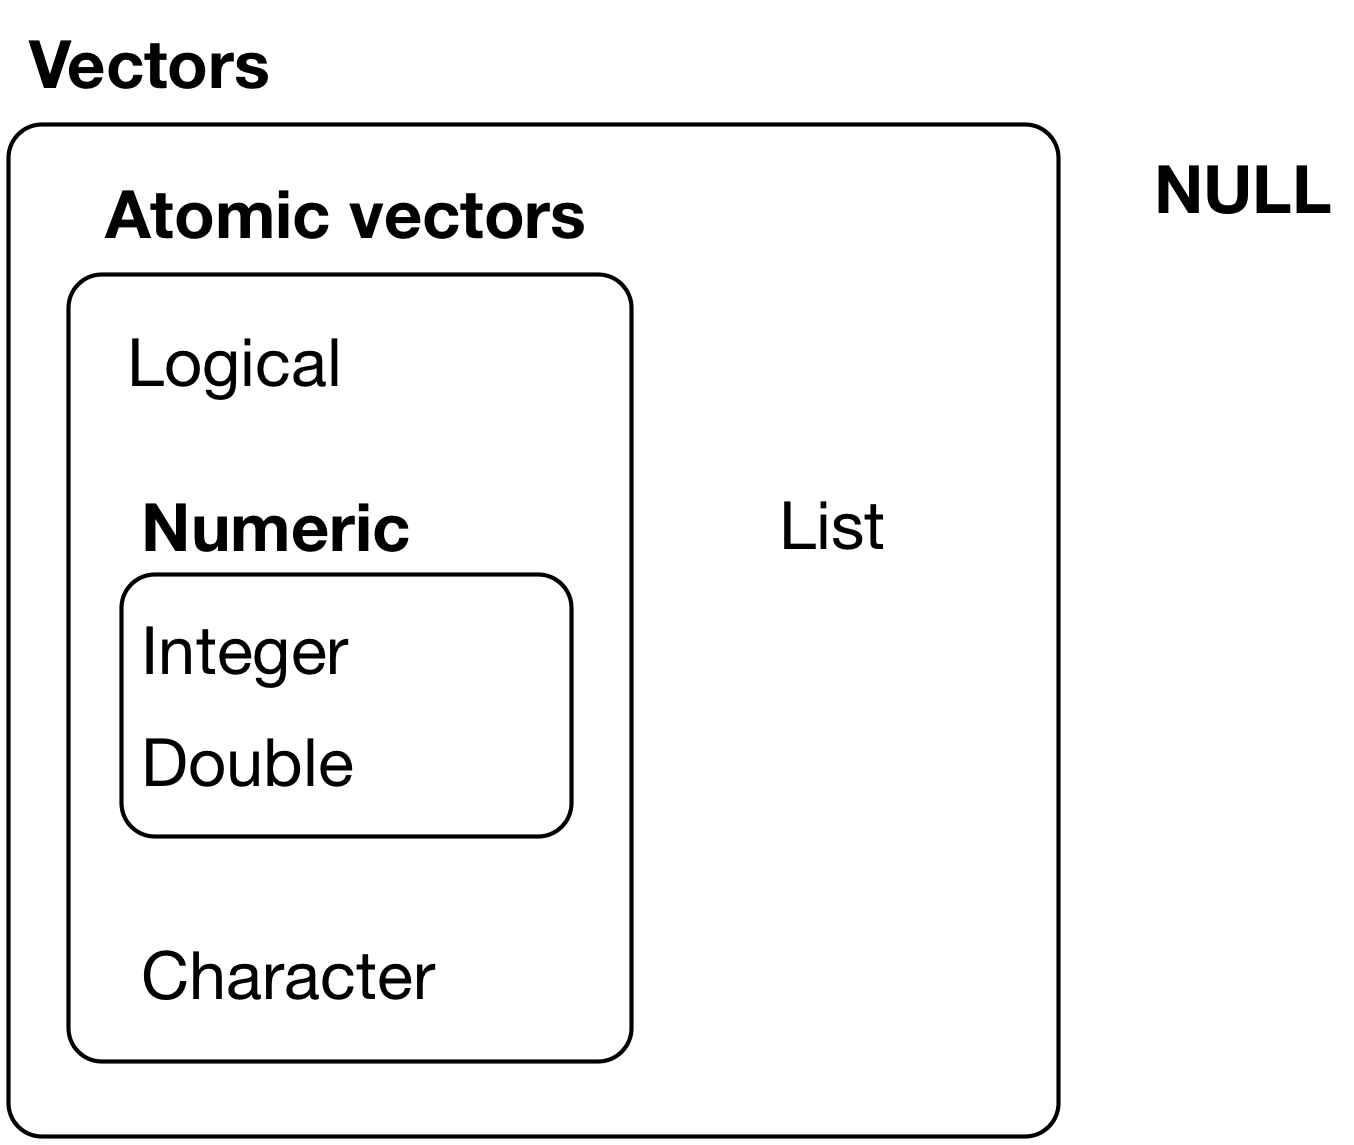
\includegraphics{../img/data-structures-overview.png}
\caption{Hierarchy of R's vector types}
\end{figure}
\end{frame}

\begin{frame}[fragile]{ベクトルのプロパティ}
\protect\hypertarget{ux30d9ux30afux30c8ux30ebux306eux30d7ux30edux30d1ux30c6ux30a3}{}
\begin{block}{型}
\protect\hypertarget{ux578b}{}
\begin{Shaded}
\begin{Highlighting}[]
\FunctionTok{typeof}\NormalTok{(}\DecValTok{1}\SpecialCharTok{:}\DecValTok{10}\NormalTok{)}
\end{Highlighting}
\end{Shaded}

\begin{verbatim}
## [1] "integer"
\end{verbatim}

\begin{Shaded}
\begin{Highlighting}[]
\FunctionTok{typeof}\NormalTok{(}\FunctionTok{list}\NormalTok{(}\DecValTok{1}\NormalTok{,}\StringTok{"a"}\NormalTok{))}
\end{Highlighting}
\end{Shaded}

\begin{verbatim}
## [1] "list"
\end{verbatim}
\end{block}

\begin{block}{長さ}
\protect\hypertarget{ux9577ux3055}{}
\begin{Shaded}
\begin{Highlighting}[]
\FunctionTok{length}\NormalTok{(}\DecValTok{1}\SpecialCharTok{:}\DecValTok{10}\NormalTok{)}
\end{Highlighting}
\end{Shaded}

\begin{verbatim}
## [1] 10
\end{verbatim}
\end{block}
\end{frame}

\begin{frame}{拡張されたベクトル}
\protect\hypertarget{ux62e1ux5f35ux3055ux308cux305fux30d9ux30afux30c8ux30eb}{}
一部のベクトルは\textbf{属性(attribute)}という付加情報を持たせて複雑な操作ができる。

\begin{itemize}
\tightlist
\item
  factor:実体はintegerベクトル
\item
  date: 実体はdoubleベクトル
\item
  data.frame: 実体はリスト
\end{itemize}
\end{frame}

\begin{frame}{20.3 Important types of atomic vector}
\protect\hypertarget{important-types-of-atomic-vector}{}
\begin{itemize}
\tightlist
\item
  logical, integer, double, character

  \begin{itemize}
  \tightlist
  \item
    complex, rawは扱わない
  \end{itemize}
\end{itemize}
\end{frame}

\begin{frame}[fragile]{20.3.1 Logical}
\protect\hypertarget{logical}{}
最も原子的

\begin{block}{値}
\protect\hypertarget{ux5024}{}
\texttt{TRUE}, \texttt{FALSE}, \texttt{NA}の三種類のみ
\end{block}

\begin{block}{生成}
\protect\hypertarget{ux751fux6210}{}
\begin{Shaded}
\begin{Highlighting}[]
\DecValTok{1}\SpecialCharTok{:}\DecValTok{10} \SpecialCharTok{\%\%} \DecValTok{3} \SpecialCharTok{==} \DecValTok{0}
\end{Highlighting}
\end{Shaded}

\begin{verbatim}
##  [1] FALSE FALSE  TRUE FALSE FALSE  TRUE FALSE FALSE  TRUE FALSE
\end{verbatim}

\begin{Shaded}
\begin{Highlighting}[]
\FunctionTok{c}\NormalTok{(}\ConstantTok{TRUE}\NormalTok{, }\ConstantTok{TRUE}\NormalTok{, }\ConstantTok{FALSE}\NormalTok{, }\ConstantTok{NA}\NormalTok{)}
\end{Highlighting}
\end{Shaded}

\begin{verbatim}
## [1]  TRUE  TRUE FALSE    NA
\end{verbatim}
\end{block}
\end{frame}

\begin{frame}[fragile]{20.3.2 Numeric}
\protect\hypertarget{numeric}{}
Logicalの次に原子的

二種類に分類できる

\begin{itemize}
\tightlist
\item
  integer
\item
  double(デフォルト)
\end{itemize}

\begin{Shaded}
\begin{Highlighting}[]
\FunctionTok{typeof}\NormalTok{(}\DecValTok{1}\NormalTok{)}
\end{Highlighting}
\end{Shaded}

\begin{verbatim}
## [1] "double"
\end{verbatim}

\begin{Shaded}
\begin{Highlighting}[]
\FunctionTok{typeof}\NormalTok{(1L)}
\end{Highlighting}
\end{Shaded}

\begin{verbatim}
## [1] "integer"
\end{verbatim}
\end{frame}

\begin{frame}[fragile]{doubleは近似}
\protect\hypertarget{doubleux306fux8fd1ux4f3c}{}
\begin{Shaded}
\begin{Highlighting}[]
\NormalTok{x }\OtherTok{\textless{}{-}} \FunctionTok{sqrt}\NormalTok{(}\DecValTok{2}\NormalTok{) }\SpecialCharTok{\^{}} \DecValTok{2}
\NormalTok{x}
\end{Highlighting}
\end{Shaded}

\begin{verbatim}
## [1] 2
\end{verbatim}

\begin{Shaded}
\begin{Highlighting}[]
\NormalTok{x }\SpecialCharTok{{-}} \DecValTok{2}
\end{Highlighting}
\end{Shaded}

\begin{verbatim}
## [1] 4.440892e-16
\end{verbatim}

\begin{block}{教訓}
\protect\hypertarget{ux6559ux8a13}{}
\texttt{==}じゃなくて\texttt{near}を使う
\end{block}
\end{frame}

\begin{frame}[fragile]{特殊な値}
\protect\hypertarget{ux7279ux6b8aux306aux5024}{}
\begin{itemize}
\tightlist
\item
  \texttt{NA}
\item
  \texttt{NaN} (doubleのみ)
\item
  \texttt{Inf}, \texttt{-Inf} (doubleのみ)
\end{itemize}

\begin{block}{check}
\protect\hypertarget{check}{}
\texttt{is.na}, \texttt{is.finite}, \texttt{is.nan}
\end{block}
\end{frame}

\begin{frame}{20.3.3 Character}
\protect\hypertarget{character}{}
\end{frame}

\begin{frame}[fragile]{Global string pool}
\protect\hypertarget{global-string-pool}{}
文字列の実体は一箇所に保管されている

\(\Rightarrow\) データの実体はpoolへのリンク

\begin{Shaded}
\begin{Highlighting}[]
\NormalTok{x }\OtherTok{\textless{}{-}} \StringTok{"This is a reasonably long string."}
\NormalTok{pryr}\SpecialCharTok{::}\FunctionTok{object\_size}\NormalTok{(x)}
\end{Highlighting}
\end{Shaded}

\begin{verbatim}
## 152 B
\end{verbatim}

\begin{Shaded}
\begin{Highlighting}[]
\NormalTok{y }\OtherTok{\textless{}{-}} \FunctionTok{rep}\NormalTok{(x, }\DecValTok{1000}\NormalTok{)}
\NormalTok{pryr}\SpecialCharTok{::}\FunctionTok{object\_size}\NormalTok{(y)}
\end{Highlighting}
\end{Shaded}

\begin{verbatim}
## 8.14 kB
\end{verbatim}
\end{frame}

\begin{frame}[fragile]{20.3.4 Missing values}
\protect\hypertarget{missing-values}{}
実は\texttt{NA}にも型が存在する

\begin{Shaded}
\begin{Highlighting}[]
\ConstantTok{NA}            \CommentTok{\# logical}
\ConstantTok{NA\_integer\_}   \CommentTok{\# integer}
\ConstantTok{NA\_real\_}      \CommentTok{\# double}
\ConstantTok{NA\_character\_} \CommentTok{\# character}
\end{Highlighting}
\end{Shaded}
\end{frame}

\begin{frame}{20.3.5 Exercises}
\protect\hypertarget{exercises}{}
\end{frame}

\begin{frame}{20.4 Using atomic vectors}
\protect\hypertarget{using-atomic-vectors}{}
\begin{enumerate}
\tightlist
\item
  どうやって型を変換するか
\item
  ベクトルの型の調べ方
\item
  異なる長さのベクトルがどのように作用するか
\item
  ベクトルの要素に名前を付ける方法
\item
  ベクトルの要素の抽出方法
\end{enumerate}
\end{frame}

\begin{frame}{20.4.1 Coercion}
\protect\hypertarget{coercion}{}
型の変換

明示的(Explicit)な方法と暗黙的(Implicit)な方法
\end{frame}

\begin{frame}[fragile]{明示的な方法}
\protect\hypertarget{ux660eux793aux7684ux306aux65b9ux6cd5}{}
関数

\begin{itemize}
\tightlist
\item
  \texttt{as.logical}
\item
  \texttt{as.integer}
\item
  \texttt{as.double}
\item
  \texttt{as.character}
\end{itemize}

logical \textgreater{} integer \textgreater{} double \textgreater{}
character

の順に変換すればとりあえず間違いない。

逆も不可能ではないけど扱いに注意
\end{frame}

\begin{frame}[fragile]{暗黙的な方法: 例1}
\protect\hypertarget{ux6697ux9ed9ux7684ux306aux65b9ux6cd5-ux4f8buxff11}{}
logicalを実数として処理する方法

\begin{Shaded}
\begin{Highlighting}[]
\NormalTok{x }\OtherTok{\textless{}{-}} \FunctionTok{sample}\NormalTok{(}\DecValTok{20}\NormalTok{, }\DecValTok{100}\NormalTok{, }\AttributeTok{replace =} \ConstantTok{TRUE}\NormalTok{)}
\FunctionTok{sum}\NormalTok{(x }\SpecialCharTok{\textgreater{}} \DecValTok{10}\NormalTok{)  }\CommentTok{\# how many are greater than 10?}
\end{Highlighting}
\end{Shaded}

\begin{verbatim}
## [1] 52
\end{verbatim}

\texttt{TRUE}は\texttt{1}に、\texttt{FALSE}は\texttt{0}になる
\end{frame}

\begin{frame}[fragile]{暗黙的な方法: 例2}
\protect\hypertarget{ux6697ux9ed9ux7684ux306aux65b9ux6cd5-ux4f8buxff12}{}
異なる型の値(ベクトル)を\texttt{c}で結合

\begin{Shaded}
\begin{Highlighting}[]
\FunctionTok{typeof}\NormalTok{(}\FunctionTok{c}\NormalTok{(}\ConstantTok{TRUE}\NormalTok{, 1L))}
\end{Highlighting}
\end{Shaded}

\begin{verbatim}
## [1] "integer"
\end{verbatim}

\begin{Shaded}
\begin{Highlighting}[]
\FunctionTok{typeof}\NormalTok{(}\FunctionTok{c}\NormalTok{(}\FloatTok{1.5}\NormalTok{, }\StringTok{"a"}\NormalTok{))}
\end{Highlighting}
\end{Shaded}

\begin{verbatim}
## [1] "character"
\end{verbatim}

logical \textless{} integer \textless{} double \textless{} complex
\textless{} character\\
の強さの順で統一される

\begin{block}{はっきりと認識しておくこと}
\protect\hypertarget{ux306fux3063ux304dux308aux3068ux8a8dux8b58ux3057ux3066ux304aux304fux3053ux3068}{}
ベクトルは複数種類の型の値を要素に持つことはできない
\end{block}
\end{frame}

\begin{frame}[fragile]{20.4.2 Test functions}
\protect\hypertarget{test-functions}{}
どの型のアトミックなのかテストする関数

\begin{longtable}[]{@{}llllll@{}}
\toprule()
& lgl & int & dbl & chr & list \\
\midrule()
\endhead
\texttt{is\_logical} & x & & & & \\
\texttt{is\_integer} & & x & & & \\
\texttt{is\_double} & & & x & & \\
\texttt{is\_numeric} & & x & x & & \\
\texttt{is\_character} & & & & x & \\
\texttt{is\_atomic} & x & x & x & x & \\
\texttt{is\_list} & & & & & x \\
\texttt{is\_vector} & x & x & x & x & x \\
\bottomrule()
\end{longtable}

\begin{block}{scalar}
\protect\hypertarget{scalar}{}
\texttt{is\_scalar\_logical}で長さ1のlglかどうかテスト
\end{block}
\end{frame}

\begin{frame}{20.4.3 Scalars and recycling rules}
\protect\hypertarget{scalars-and-recycling-rules}{}
アトミックベクトルどうしの演算
\end{frame}

\begin{frame}[fragile]{基本ルール}
\protect\hypertarget{ux57faux672cux30ebux30fcux30eb}{}
要素ごとに演算される

\begin{Shaded}
\begin{Highlighting}[]
\FunctionTok{c}\NormalTok{(}\DecValTok{1}\NormalTok{, }\DecValTok{2}\NormalTok{, }\DecValTok{3}\NormalTok{) }\SpecialCharTok{*} \FunctionTok{c}\NormalTok{(}\DecValTok{1}\NormalTok{, }\DecValTok{10}\NormalTok{, }\DecValTok{100}\NormalTok{)}
\end{Highlighting}
\end{Shaded}

\begin{verbatim}
## [1]   1  20 300
\end{verbatim}

長さが違う場合は?
\end{frame}

\begin{frame}[fragile]{リサイクル}
\protect\hypertarget{ux30eaux30b5ux30a4ux30afux30eb}{}
演算入力のベクトルの長さが異なる場合は短い方が繰り返される

\begin{Shaded}
\begin{Highlighting}[]
\DecValTok{1}\SpecialCharTok{:}\DecValTok{10} \SpecialCharTok{+} \DecValTok{100}
\end{Highlighting}
\end{Shaded}

\begin{verbatim}
##  [1] 101 102 103 104 105 106 107 108 109 110
\end{verbatim}

\begin{Shaded}
\begin{Highlighting}[]
\DecValTok{1}\SpecialCharTok{:}\DecValTok{10} \SpecialCharTok{+} \DecValTok{1}\SpecialCharTok{:}\DecValTok{2} \SpecialCharTok{*} \DecValTok{100}
\end{Highlighting}
\end{Shaded}

\begin{verbatim}
##  [1] 101 202 103 204 105 206 107 208 109 210
\end{verbatim}
\end{frame}

\begin{frame}[fragile]{リサイクル2}
\protect\hypertarget{ux30eaux30b5ux30a4ux30afux30ebuxff12}{}
繰り返し回数が合わなければ途中までリサイクル

\begin{Shaded}
\begin{Highlighting}[]
\DecValTok{1}\SpecialCharTok{:}\DecValTok{10} \SpecialCharTok{+} \DecValTok{1}\SpecialCharTok{:}\DecValTok{3} \SpecialCharTok{*} \DecValTok{100}
\end{Highlighting}
\end{Shaded}

\begin{verbatim}
## Warning in 1:10 + 1:3 * 100: 長いオブジェクトの長さが短いオブジェクトの長さの倍
## 数になっていません
\end{verbatim}

\begin{verbatim}
##  [1] 101 202 303 104 205 306 107 208 309 110
\end{verbatim}
\end{frame}

\begin{frame}[fragile]{\texttt{tidyverse}}
\protect\hypertarget{tidyverse}{}
\texttt{tidyverse}な世界ではベクトル-スカラー以外のリサイクルは禁止

\begin{Shaded}
\begin{Highlighting}[]
\FunctionTok{tibble}\NormalTok{(}\AttributeTok{x =} \DecValTok{1}\SpecialCharTok{:}\DecValTok{3}\NormalTok{, }\AttributeTok{y =} \DecValTok{1}\NormalTok{)}
\end{Highlighting}
\end{Shaded}

\begin{verbatim}
## # A tibble: 3 x 2
##       x     y
##   <int> <dbl>
## 1     1     1
## 2     2     1
## 3     3     1
\end{verbatim}

\begin{Shaded}
\begin{Highlighting}[]
\FunctionTok{tibble}\NormalTok{(}\AttributeTok{x =} \DecValTok{1}\SpecialCharTok{:}\DecValTok{3}\NormalTok{, }\AttributeTok{y =} \DecValTok{1}\SpecialCharTok{:}\DecValTok{2}\NormalTok{)}
\end{Highlighting}
\end{Shaded}

\begin{verbatim}
## Error:
## ! Tibble columns must have compatible sizes.
## * Size 3: Existing data.
## * Size 2: Column `y`.
## i Only values of size one are recycled.
\end{verbatim}
\end{frame}

\begin{frame}{20.4.4 Naming vectors}
\protect\hypertarget{naming-vectors}{}
ベクトル要素に名前をつける
\end{frame}

\begin{frame}[fragile]{ベクトル要素の名前}
\protect\hypertarget{ux30d9ux30afux30c8ux30ebux8981ux7d20ux306eux540dux524d}{}
\begin{Shaded}
\begin{Highlighting}[]
\NormalTok{v }\OtherTok{\textless{}{-}} \FunctionTok{c}\NormalTok{(}\AttributeTok{x =} \DecValTok{1}\NormalTok{, }\AttributeTok{y =} \DecValTok{2}\NormalTok{, }\AttributeTok{z =} \DecValTok{4}\NormalTok{)}
\NormalTok{v}
\end{Highlighting}
\end{Shaded}

\begin{verbatim}
## x y z 
## 1 2 4
\end{verbatim}

\begin{Shaded}
\begin{Highlighting}[]
\FunctionTok{names}\NormalTok{(v)}
\end{Highlighting}
\end{Shaded}

\begin{verbatim}
## [1] "x" "y" "z"
\end{verbatim}
\end{frame}

\begin{frame}[fragile]{名前の変更}
\protect\hypertarget{ux540dux524dux306eux5909ux66f4}{}
\begin{Shaded}
\begin{Highlighting}[]
\NormalTok{v }\SpecialCharTok{\%\textgreater{}\%} \FunctionTok{set\_names}\NormalTok{(}\FunctionTok{c}\NormalTok{(}\StringTok{"a"}\NormalTok{, }\StringTok{"b"}\NormalTok{, }\StringTok{"c"}\NormalTok{))}
\end{Highlighting}
\end{Shaded}

\begin{verbatim}
## a b c 
## 1 2 4
\end{verbatim}
\end{frame}

\begin{frame}[fragile]{20.4.5 Subsetting}
\protect\hypertarget{subsetting}{}
ベクトルの一部の要素を抽出する

\begin{block}{operator}
\protect\hypertarget{operator}{}
ベクトルの後ろに\texttt{{[}...{]}}を付ける

\texttt{{[}...{]}}の中に入れる値は三種類

\begin{itemize}
\tightlist
\item
  index
\item
  logical
\item
  name strings
\end{itemize}
\end{block}
\end{frame}

\begin{frame}[fragile]{index}
\protect\hypertarget{index}{}
前から数えた位置で指定する

\begin{Shaded}
\begin{Highlighting}[]
\NormalTok{x }\OtherTok{\textless{}{-}} \FunctionTok{c}\NormalTok{(}\StringTok{"one"}\NormalTok{, }\StringTok{"two"}\NormalTok{, }\StringTok{"three"}\NormalTok{, }\StringTok{"four"}\NormalTok{, }\StringTok{"five"}\NormalTok{)}
\NormalTok{x[}\FunctionTok{c}\NormalTok{(}\DecValTok{3}\NormalTok{, }\DecValTok{2}\NormalTok{, }\DecValTok{5}\NormalTok{)] }
\end{Highlighting}
\end{Shaded}

\begin{verbatim}
## [1] "three" "two"   "five"
\end{verbatim}

\begin{Shaded}
\begin{Highlighting}[]
\NormalTok{x[}\FunctionTok{c}\NormalTok{(}\DecValTok{1}\NormalTok{, }\DecValTok{1}\NormalTok{, }\DecValTok{5}\NormalTok{, }\DecValTok{5}\NormalTok{, }\DecValTok{5}\NormalTok{, }\DecValTok{2}\NormalTok{)] }\CommentTok{\#繰り返し}
\end{Highlighting}
\end{Shaded}

\begin{verbatim}
## [1] "one"  "one"  "five" "five" "five" "two"
\end{verbatim}

\begin{Shaded}
\begin{Highlighting}[]
\NormalTok{x[}\FunctionTok{c}\NormalTok{(}\SpecialCharTok{{-}}\DecValTok{1}\NormalTok{, }\SpecialCharTok{{-}}\DecValTok{3}\NormalTok{, }\SpecialCharTok{{-}}\DecValTok{5}\NormalTok{)] }\CommentTok{\#マイナス指定}
\end{Highlighting}
\end{Shaded}

\begin{verbatim}
## [1] "two"  "four"
\end{verbatim}
\end{frame}

\begin{frame}[fragile]{logical}
\protect\hypertarget{logical-1}{}
元と同じ長さの論理ベクトルの\texttt{TRUE}の位置で指定

\begin{Shaded}
\begin{Highlighting}[]
\NormalTok{x }\OtherTok{\textless{}{-}} \FunctionTok{c}\NormalTok{(}\DecValTok{10}\NormalTok{, }\DecValTok{3}\NormalTok{, }\ConstantTok{NA}\NormalTok{, }\DecValTok{5}\NormalTok{, }\DecValTok{8}\NormalTok{, }\DecValTok{1}\NormalTok{, }\ConstantTok{NA}\NormalTok{)}
\NormalTok{x[}\SpecialCharTok{!}\FunctionTok{is.na}\NormalTok{(x)] }\CommentTok{\#NAを除く}
\end{Highlighting}
\end{Shaded}

\begin{verbatim}
## [1] 10  3  5  8  1
\end{verbatim}

\begin{Shaded}
\begin{Highlighting}[]
\NormalTok{x[x }\SpecialCharTok{\%\%} \DecValTok{2} \SpecialCharTok{==} \DecValTok{0}\NormalTok{] }\CommentTok{\#偶数とNA}
\end{Highlighting}
\end{Shaded}

\begin{verbatim}
## [1] 10 NA  8 NA
\end{verbatim}
\end{frame}

\begin{frame}[fragile]{name strings}
\protect\hypertarget{name-strings}{}
ベクトル要素の名前で指定

\begin{Shaded}
\begin{Highlighting}[]
\NormalTok{x }\OtherTok{\textless{}{-}} \FunctionTok{c}\NormalTok{(}\AttributeTok{abc =} \DecValTok{1}\NormalTok{, }\AttributeTok{def =} \DecValTok{2}\NormalTok{, }\AttributeTok{xyz =} \DecValTok{5}\NormalTok{)}
\NormalTok{x[}\FunctionTok{c}\NormalTok{(}\StringTok{"xyz"}\NormalTok{, }\StringTok{"def"}\NormalTok{)]}
\end{Highlighting}
\end{Shaded}

\begin{verbatim}
## xyz def 
##   5   2
\end{verbatim}
\end{frame}

\begin{frame}[fragile]{nothing}
\protect\hypertarget{nothing}{}
要素を指定せずに全体を得る

\begin{Shaded}
\begin{Highlighting}[]
\NormalTok{iris[}\DecValTok{1}\NormalTok{,]}
\end{Highlighting}
\end{Shaded}

\begin{verbatim}
##   Sepal.Length Sepal.Width Petal.Length Petal.Width Species
## 1          5.1         3.5          1.4         0.2  setosa
\end{verbatim}

\begin{Shaded}
\begin{Highlighting}[]
\NormalTok{iris[,}\DecValTok{1}\NormalTok{]}
\end{Highlighting}
\end{Shaded}

\begin{verbatim}
##   [1] 5.1 4.9 4.7 4.6 5.0 5.4 4.6 5.0 4.4 4.9 5.4 4.8 4.8 4.3 5.8 5.7 5.4 5.1
##  [19] 5.7 5.1 5.4 5.1 4.6 5.1 4.8 5.0 5.0 5.2 5.2 4.7 4.8 5.4 5.2 5.5 4.9 5.0
##  [37] 5.5 4.9 4.4 5.1 5.0 4.5 4.4 5.0 5.1 4.8 5.1 4.6 5.3 5.0 7.0 6.4 6.9 5.5
##  [55] 6.5 5.7 6.3 4.9 6.6 5.2 5.0 5.9 6.0 6.1 5.6 6.7 5.6 5.8 6.2 5.6 5.9 6.1
##  [73] 6.3 6.1 6.4 6.6 6.8 6.7 6.0 5.7 5.5 5.5 5.8 6.0 5.4 6.0 6.7 6.3 5.6 5.5
##  [91] 5.5 6.1 5.8 5.0 5.6 5.7 5.7 6.2 5.1 5.7 6.3 5.8 7.1 6.3 6.5 7.6 4.9 7.3
## [109] 6.7 7.2 6.5 6.4 6.8 5.7 5.8 6.4 6.5 7.7 7.7 6.0 6.9 5.6 7.7 6.3 6.7 7.2
## [127] 6.2 6.1 6.4 7.2 7.4 7.9 6.4 6.3 6.1 7.7 6.3 6.4 6.0 6.9 6.7 6.9 5.8 6.8
## [145] 6.7 6.7 6.3 6.5 6.2 5.9
\end{verbatim}
\end{frame}

\begin{frame}[fragile]{subsetting function}
\protect\hypertarget{subsetting-function}{}
実は関数\texttt{"{[}"}がコールされている

\begin{Shaded}
\begin{Highlighting}[]
\StringTok{"["}\NormalTok{(x, }\DecValTok{1}\NormalTok{)}
\end{Highlighting}
\end{Shaded}

\begin{verbatim}
## abc 
##   1
\end{verbatim}

\begin{Shaded}
\begin{Highlighting}[]
\NormalTok{x }\SpecialCharTok{\%\textgreater{}\%} \StringTok{"["}\NormalTok{(}\DecValTok{1}\NormalTok{)}
\end{Highlighting}
\end{Shaded}

\begin{verbatim}
## abc 
##   1
\end{verbatim}
\end{frame}

\begin{frame}{20.4.6 Exercises}
\protect\hypertarget{exercises-1}{}
\end{frame}

\begin{frame}{20.5 Recursive vectors (lists)}
\protect\hypertarget{recursive-vectors-lists}{}
制約が無さ過ぎるベクトル
\end{frame}

\begin{frame}[fragile]{型の制約なし}
\protect\hypertarget{ux578bux306eux5236ux7d04ux306aux3057}{}
アトミックのように要素の型が統一されている必要がない

\begin{Shaded}
\begin{Highlighting}[]
\NormalTok{y }\OtherTok{\textless{}{-}} \FunctionTok{list}\NormalTok{(}\StringTok{"a"}\NormalTok{, 1L, }\FloatTok{1.5}\NormalTok{, }\ConstantTok{TRUE}\NormalTok{)}
\FunctionTok{str}\NormalTok{(y)}
\end{Highlighting}
\end{Shaded}

\begin{verbatim}
## List of 4
##  $ : chr "a"
##  $ : int 1
##  $ : num 1.5
##  $ : logi TRUE
\end{verbatim}
\end{frame}

\begin{frame}[fragile]{繰り返し}
\protect\hypertarget{ux7e70ux308aux8fd4ux3057}{}
listはlistを要素に持てる

\begin{Shaded}
\begin{Highlighting}[]
\NormalTok{z }\OtherTok{\textless{}{-}} \FunctionTok{list}\NormalTok{(}\FunctionTok{list}\NormalTok{(}\DecValTok{1}\NormalTok{, }\DecValTok{2}\NormalTok{), }\FunctionTok{list}\NormalTok{(}\DecValTok{3}\NormalTok{, }\DecValTok{4}\NormalTok{, }\DecValTok{5}\NormalTok{))}
\FunctionTok{str}\NormalTok{(z)}
\end{Highlighting}
\end{Shaded}

\begin{verbatim}
## List of 2
##  $ :List of 2
##   ..$ : num 1
##   ..$ : num 2
##  $ :List of 3
##   ..$ : num 3
##   ..$ : num 4
##   ..$ : num 5
\end{verbatim}
\end{frame}

\begin{frame}{20.5.1 Visualising lists}
\protect\hypertarget{visualising-lists}{}
list構造の可視化方法

この本のためのHadleyさんオリジナル
\end{frame}

\begin{frame}[fragile]{リストの可視化ルール}
\protect\hypertarget{ux30eaux30b9ux30c8ux306eux53efux8996ux5316ux30ebux30fcux30eb}{}
\begin{Shaded}
\begin{Highlighting}[]
\NormalTok{x1 }\OtherTok{\textless{}{-}} \FunctionTok{list}\NormalTok{(}\FunctionTok{c}\NormalTok{(}\DecValTok{1}\NormalTok{, }\DecValTok{2}\NormalTok{), }\FunctionTok{c}\NormalTok{(}\DecValTok{3}\NormalTok{, }\DecValTok{4}\NormalTok{))}
\NormalTok{x2 }\OtherTok{\textless{}{-}} \FunctionTok{list}\NormalTok{(}\FunctionTok{list}\NormalTok{(}\DecValTok{1}\NormalTok{, }\DecValTok{2}\NormalTok{), }\FunctionTok{list}\NormalTok{(}\DecValTok{3}\NormalTok{, }\DecValTok{4}\NormalTok{))}
\NormalTok{x3 }\OtherTok{\textless{}{-}} \FunctionTok{list}\NormalTok{(}\DecValTok{1}\NormalTok{, }\FunctionTok{list}\NormalTok{(}\DecValTok{2}\NormalTok{, }\FunctionTok{list}\NormalTok{(}\DecValTok{3}\NormalTok{)))}
\end{Highlighting}
\end{Shaded}

\begin{center}
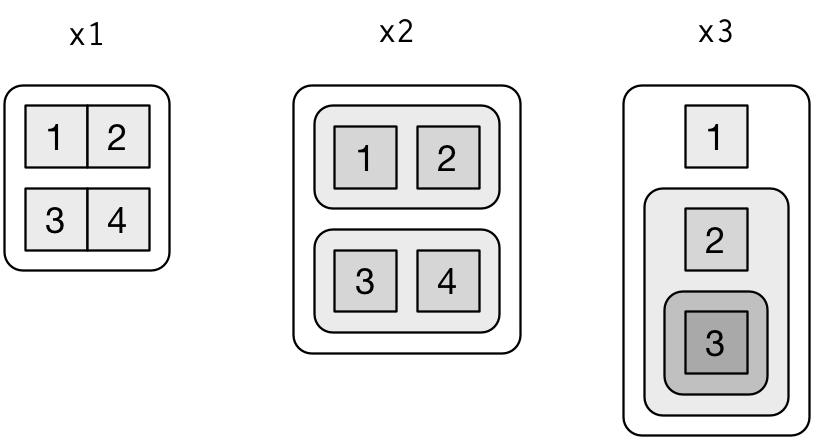
\includegraphics[width=80mm]{../img/lists-structure.png}
\end{center}

\begin{itemize}
\tightlist
\item
  リストは角が丸、アトミックは四角
\item
  子は親の中に入れる。階層が深いとグレー
\item
  向きや順序に意味はない
\end{itemize}
\end{frame}

\begin{frame}[fragile]{20.5.2 Subsetting}
\protect\hypertarget{subsetting-1}{}
リストには三種の要素抽出方法がある

\begin{Shaded}
\begin{Highlighting}[]
\NormalTok{a }\OtherTok{\textless{}{-}} \FunctionTok{list}\NormalTok{(}\AttributeTok{a =} \DecValTok{1}\SpecialCharTok{:}\DecValTok{3}\NormalTok{, }\AttributeTok{b =} \StringTok{"a string"}\NormalTok{, }\AttributeTok{c =}\NormalTok{ pi, }\AttributeTok{d =} \FunctionTok{list}\NormalTok{(}\SpecialCharTok{{-}}\DecValTok{1}\NormalTok{, }\SpecialCharTok{{-}}\DecValTok{5}\NormalTok{))}
\NormalTok{a[}\DecValTok{1}\NormalTok{]}
\end{Highlighting}
\end{Shaded}

\begin{verbatim}
## $a
## [1] 1 2 3
\end{verbatim}

\begin{Shaded}
\begin{Highlighting}[]
\NormalTok{a[[}\DecValTok{1}\NormalTok{]]}
\end{Highlighting}
\end{Shaded}

\begin{verbatim}
## [1] 1 2 3
\end{verbatim}

\begin{Shaded}
\begin{Highlighting}[]
\NormalTok{a}\SpecialCharTok{$}\NormalTok{a}
\end{Highlighting}
\end{Shaded}

\begin{verbatim}
## [1] 1 2 3
\end{verbatim}
\end{frame}

\begin{frame}{可視化}
\protect\hypertarget{ux53efux8996ux5316}{}
\begin{figure}
\centering
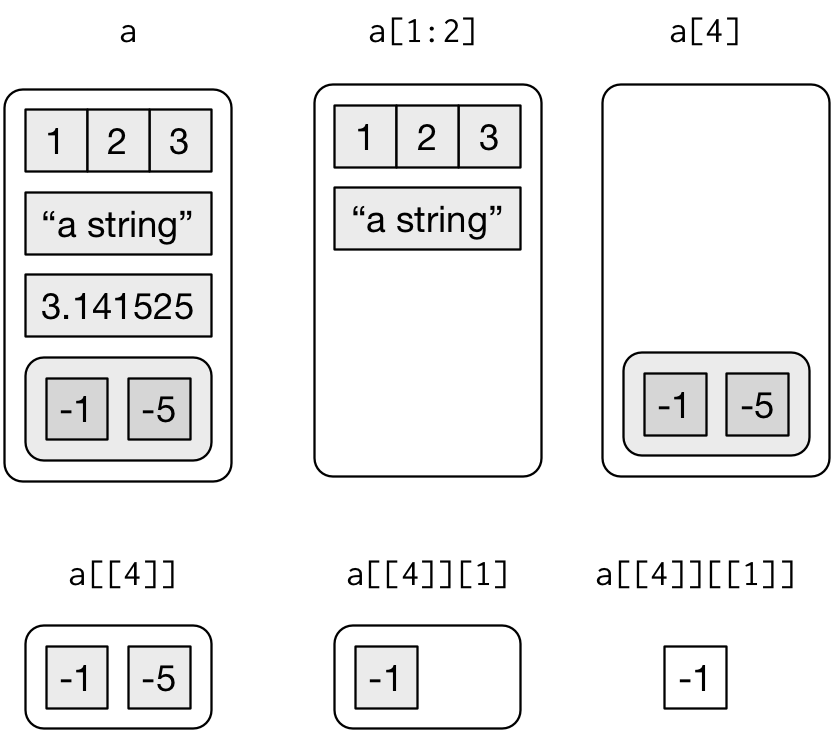
\includegraphics[width=0.8\textwidth,height=\textheight]{../img/lists-subsetting.png}
\caption{Subsetting a list, visually}
\end{figure}
\end{frame}

\begin{frame}[fragile]{20.5.3 Lists of condiments}
\protect\hypertarget{lists-of-condiments}{}
たとえ話

\begin{longtable}[]{@{}
  >{\centering\arraybackslash}p{(\columnwidth - 6\tabcolsep) * \real{0.2500}}
  >{\centering\arraybackslash}p{(\columnwidth - 6\tabcolsep) * \real{0.2500}}
  >{\centering\arraybackslash}p{(\columnwidth - 6\tabcolsep) * \real{0.2500}}
  >{\centering\arraybackslash}p{(\columnwidth - 6\tabcolsep) * \real{0.2500}}@{}}
\toprule()
\begin{minipage}[b]{\linewidth}\centering
\texttt{a}
\end{minipage} & \begin{minipage}[b]{\linewidth}\centering
\texttt{a{[}1{]}}
\end{minipage} & \begin{minipage}[b]{\linewidth}\centering
\texttt{a{[}{[}1{]}{]}}
\end{minipage} & \begin{minipage}[b]{\linewidth}\centering
\texttt{a{[}{[}1{]}{]}{[}{[}1{]}{]}}
\end{minipage} \\
\midrule()
\endhead

\includegraphics[width=0.2\textwidth,height=\textheight]{../img/pepper.jpg}
&
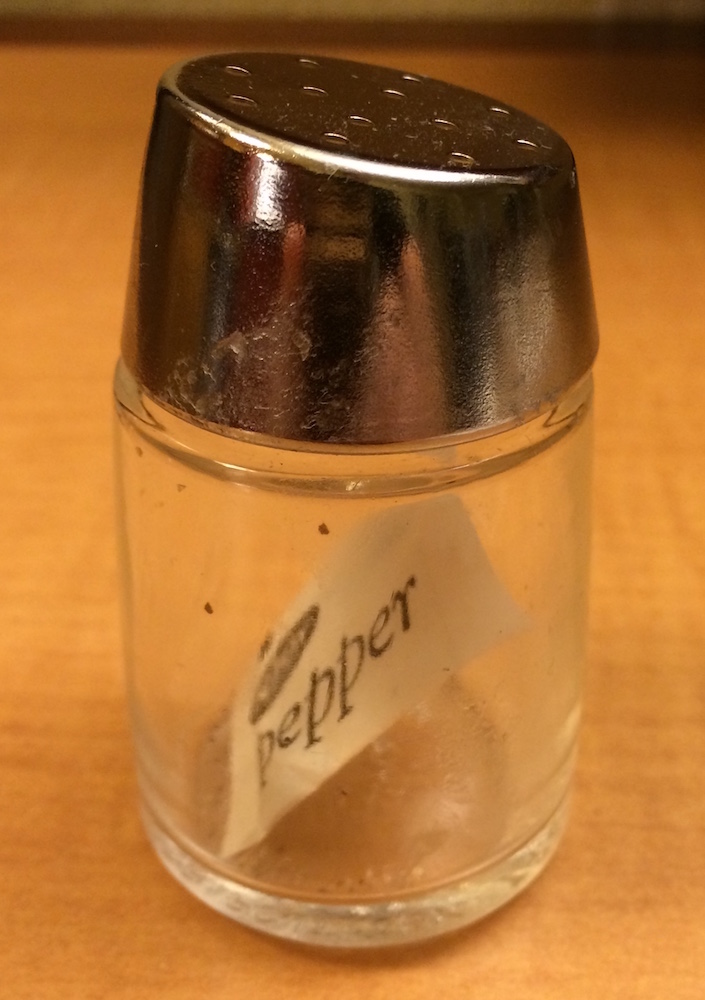
\includegraphics[width=0.2\textwidth,height=\textheight]{../img/pepper-1.jpg}
&
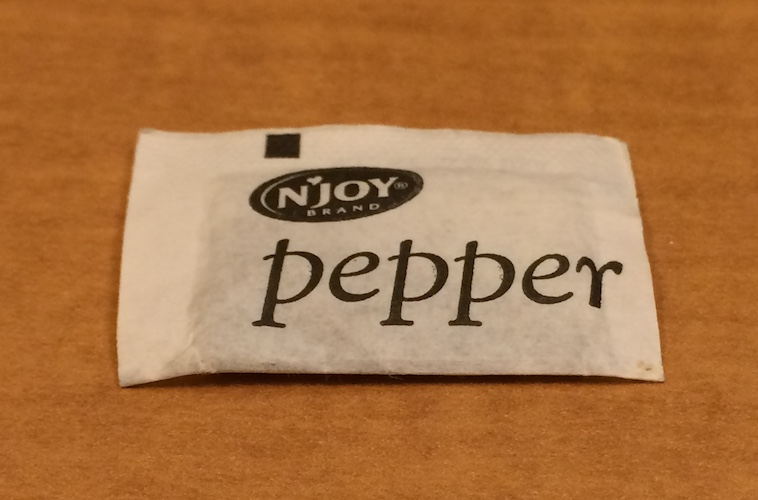
\includegraphics[width=0.2\textwidth,height=\textheight]{../img/pepper-2.jpg}
&
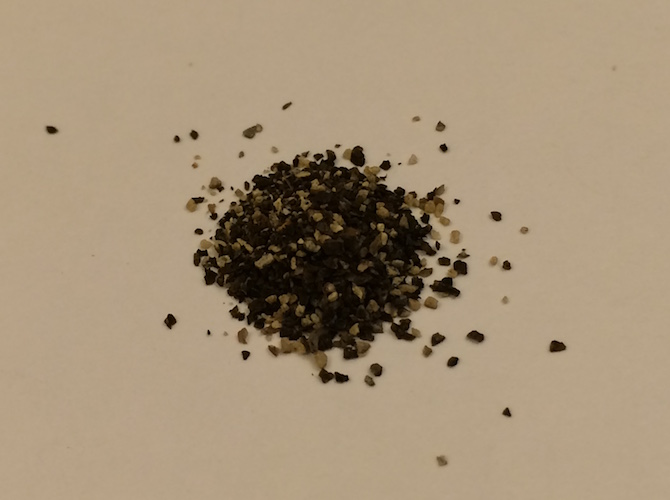
\includegraphics[width=0.2\textwidth,height=\textheight]{../img/pepper-3.jpg} \\
\bottomrule()
\end{longtable}
\end{frame}

\begin{frame}{20.5.4 Exercises}
\protect\hypertarget{exercises-2}{}
\end{frame}

\begin{frame}{20.6 Attributes}
\protect\hypertarget{attributes}{}
ベクトルの属性(付加的な情報)
\end{frame}

\begin{frame}[fragile]{設定方法}
\protect\hypertarget{ux8a2dux5b9aux65b9ux6cd5}{}
\begin{Shaded}
\begin{Highlighting}[]
\NormalTok{x }\OtherTok{\textless{}{-}} \DecValTok{1}\SpecialCharTok{:}\DecValTok{10}
\FunctionTok{attr}\NormalTok{(x, }\StringTok{"greeting"}\NormalTok{)}
\end{Highlighting}
\end{Shaded}

\begin{verbatim}
## NULL
\end{verbatim}

\begin{Shaded}
\begin{Highlighting}[]
\FunctionTok{attr}\NormalTok{(x, }\StringTok{"greeting"}\NormalTok{) }\OtherTok{\textless{}{-}} \StringTok{"Hi!"}
\FunctionTok{attr}\NormalTok{(x, }\StringTok{"farewell"}\NormalTok{) }\OtherTok{\textless{}{-}} \StringTok{"Bye!"}
\FunctionTok{attributes}\NormalTok{(x)}
\end{Highlighting}
\end{Shaded}

\begin{verbatim}
## $greeting
## [1] "Hi!"
## 
## $farewell
## [1] "Bye!"
\end{verbatim}
\end{frame}

\begin{frame}{重要な属性}
\protect\hypertarget{ux91cdux8981ux306aux5c5eux6027}{}
\begin{enumerate}
\tightlist
\item
  names: 要素の名前
\item
  dimensions: 横や縦の次元を与えればベクトルを行列にできる
\item
  class: S3オブジェクト指向プログラミングのために使う

  \begin{itemize}
  \tightlist
  \item
    汎用関数の作用を制御する
  \end{itemize}
\end{enumerate}
\end{frame}

\begin{frame}[fragile]{汎用関数の例}
\protect\hypertarget{ux6c4eux7528ux95a2ux6570ux306eux4f8b}{}
\begin{Shaded}
\begin{Highlighting}[]
\FunctionTok{as.Date}\NormalTok{(}\StringTok{"2019/8/20"}\NormalTok{)}
\end{Highlighting}
\end{Shaded}

\begin{verbatim}
## [1] "2019-08-20"
\end{verbatim}

\begin{Shaded}
\begin{Highlighting}[]
\FunctionTok{as.Date}\NormalTok{(}\DecValTok{18128}\NormalTok{)}
\end{Highlighting}
\end{Shaded}

\begin{verbatim}
## Error in as.Date.numeric(18128):  'origin' を指定しなければなりません
\end{verbatim}
\end{frame}

\begin{frame}[fragile]{もう一つの例}
\protect\hypertarget{ux3082ux3046ux4e00ux3064ux306eux4f8b}{}
\begin{Shaded}
\begin{Highlighting}[]
\FunctionTok{par}\NormalTok{(}\AttributeTok{mfrow =} \FunctionTok{c}\NormalTok{(}\DecValTok{1}\NormalTok{,}\DecValTok{2}\NormalTok{))}
\FunctionTok{plot}\NormalTok{(cars)}
\FunctionTok{plot}\NormalTok{(}\FunctionTok{lm}\NormalTok{(dist }\SpecialCharTok{\textasciitilde{}}\NormalTok{ speed, cars))}
\end{Highlighting}
\end{Shaded}

\includegraphics{ch20_vectors_files/figure-beamer/generic.plot-1.pdf}
\includegraphics{ch20_vectors_files/figure-beamer/generic.plot-2.pdf}
\includegraphics{ch20_vectors_files/figure-beamer/generic.plot-3.pdf}
\end{frame}

\begin{frame}{20.7 Augmented vectors}
\protect\hypertarget{augmented-vectors}{}
attributesの実践的な活用例

\begin{itemize}
\tightlist
\item
  factor
\item
  dates
\item
  datetimes
\item
  tibbles
\end{itemize}
\end{frame}

\begin{frame}[fragile]{20.7.1 Factors}
\protect\hypertarget{factors}{}
\begin{Shaded}
\begin{Highlighting}[]
\NormalTok{x }\OtherTok{\textless{}{-}} \FunctionTok{factor}\NormalTok{(}\FunctionTok{c}\NormalTok{(}\StringTok{"ab"}\NormalTok{, }\StringTok{"cd"}\NormalTok{, }\StringTok{"ab"}\NormalTok{), }\AttributeTok{levels =} \FunctionTok{c}\NormalTok{(}\StringTok{"ab"}\NormalTok{, }\StringTok{"cd"}\NormalTok{, }\StringTok{"ef"}\NormalTok{))}
\FunctionTok{typeof}\NormalTok{(x)}
\end{Highlighting}
\end{Shaded}

\begin{verbatim}
## [1] "integer"
\end{verbatim}

\begin{Shaded}
\begin{Highlighting}[]
\FunctionTok{attributes}\NormalTok{(x)}
\end{Highlighting}
\end{Shaded}

\begin{verbatim}
## $levels
## [1] "ab" "cd" "ef"
## 
## $class
## [1] "factor"
\end{verbatim}
\end{frame}

\begin{frame}[fragile]{20.7.2 Dates and datetimes}
\protect\hypertarget{dates-and-datetimes}{}
\begin{block}{date}
\protect\hypertarget{date}{}
\begin{Shaded}
\begin{Highlighting}[]
\NormalTok{x }\OtherTok{\textless{}{-}} \FunctionTok{as.Date}\NormalTok{(}\StringTok{"1971{-}01{-}01"}\NormalTok{)}
\FunctionTok{unclass}\NormalTok{(x)}
\end{Highlighting}
\end{Shaded}

\begin{verbatim}
## [1] 365
\end{verbatim}

\begin{Shaded}
\begin{Highlighting}[]
\FunctionTok{typeof}\NormalTok{(x)}
\end{Highlighting}
\end{Shaded}

\begin{verbatim}
## [1] "double"
\end{verbatim}

\begin{Shaded}
\begin{Highlighting}[]
\FunctionTok{attributes}\NormalTok{(x)}
\end{Highlighting}
\end{Shaded}

\begin{verbatim}
## $class
## [1] "Date"
\end{verbatim}
\end{block}
\end{frame}

\begin{frame}[fragile]{datetime}
\protect\hypertarget{datetime}{}
\begin{Shaded}
\begin{Highlighting}[]
\NormalTok{x }\OtherTok{\textless{}{-}}\NormalTok{ lubridate}\SpecialCharTok{::}\FunctionTok{ymd\_hm}\NormalTok{(}\StringTok{"1970{-}01{-}01 01:00"}\NormalTok{)}
\FunctionTok{typeof}\NormalTok{(x)}
\end{Highlighting}
\end{Shaded}

\begin{verbatim}
## [1] "double"
\end{verbatim}

\begin{Shaded}
\begin{Highlighting}[]
\FunctionTok{attributes}\NormalTok{(x)}
\end{Highlighting}
\end{Shaded}

\begin{verbatim}
## $class
## [1] "POSIXct" "POSIXt" 
## 
## $tzone
## [1] "UTC"
\end{verbatim}
\end{frame}

\begin{frame}[fragile]{update attribute}
\protect\hypertarget{update-attribute}{}
\begin{Shaded}
\begin{Highlighting}[]
\FunctionTok{attr}\NormalTok{(x, }\StringTok{"tzone"}\NormalTok{) }\OtherTok{\textless{}{-}} \StringTok{"US/Pacific"}
\NormalTok{x}
\end{Highlighting}
\end{Shaded}

\begin{verbatim}
## [1] "1969-12-31 17:00:00 PST"
\end{verbatim}

\begin{Shaded}
\begin{Highlighting}[]
\FunctionTok{attr}\NormalTok{(x, }\StringTok{"tzone"}\NormalTok{) }\OtherTok{\textless{}{-}} \StringTok{"US/Eastern"}
\NormalTok{x}
\end{Highlighting}
\end{Shaded}

\begin{verbatim}
## [1] "1969-12-31 20:00:00 EST"
\end{verbatim}
\end{frame}

\begin{frame}[fragile]{20.7.3 Tibbles}
\protect\hypertarget{tibbles}{}
\begin{Shaded}
\begin{Highlighting}[]
\NormalTok{tb }\OtherTok{\textless{}{-}}\NormalTok{ tibble}\SpecialCharTok{::}\FunctionTok{tibble}\NormalTok{(}\AttributeTok{x =} \DecValTok{1}\SpecialCharTok{:}\DecValTok{5}\NormalTok{, }\AttributeTok{y =} \DecValTok{5}\SpecialCharTok{:}\DecValTok{1}\NormalTok{)}
\FunctionTok{typeof}\NormalTok{(tb)}
\end{Highlighting}
\end{Shaded}

\begin{verbatim}
## [1] "list"
\end{verbatim}

\begin{Shaded}
\begin{Highlighting}[]
\FunctionTok{attributes}\NormalTok{(tb)}
\end{Highlighting}
\end{Shaded}

\begin{verbatim}
## $class
## [1] "tbl_df"     "tbl"        "data.frame"
## 
## $row.names
## [1] 1 2 3 4 5
## 
## $names
## [1] "x" "y"
\end{verbatim}
\end{frame}

\begin{frame}[fragile]{dataframe}
\protect\hypertarget{dataframe}{}
\begin{Shaded}
\begin{Highlighting}[]
\NormalTok{df }\OtherTok{\textless{}{-}} \FunctionTok{data.frame}\NormalTok{(}\AttributeTok{x =} \DecValTok{1}\SpecialCharTok{:}\DecValTok{5}\NormalTok{, }\AttributeTok{y =} \DecValTok{5}\SpecialCharTok{:}\DecValTok{1}\NormalTok{)}
\FunctionTok{typeof}\NormalTok{(df)}
\end{Highlighting}
\end{Shaded}

\begin{verbatim}
## [1] "list"
\end{verbatim}

\begin{Shaded}
\begin{Highlighting}[]
\FunctionTok{attributes}\NormalTok{(df)}
\end{Highlighting}
\end{Shaded}

\begin{verbatim}
## $names
## [1] "x" "y"
## 
## $class
## [1] "data.frame"
## 
## $row.names
## [1] 1 2 3 4 5
\end{verbatim}
\end{frame}

\begin{frame}{20.7.4 Exercises}
\protect\hypertarget{exercises-3}{}
\end{frame}

\begin{frame}{参考文献}
\protect\hypertarget{ux53c2ux8003ux6587ux732e}{}
\begin{itemize}
\tightlist
\item
  \url{http://adv-r.had.co.nz/Functions.html\#lazy-evaluation}
\item
  \url{http://adv-r.had.co.nz/Subsetting.html\#applications}
\item
  \url{http://adv-r.had.co.nz/OO-essentials.html\#s3}
\end{itemize}
\end{frame}

\end{document}
